%==============================================================================
% short introduction to get template running on WINDOWS
% further explanation can be found in the pptx
% can be removed after first compilation 
%
% install MikTeX (http://www.miktex.org) - activate auto-install of packages
% install ActivePerl (https://www.perl.org/) - add to HOME
% system reboot
%
% use command-line or IDE in admin-mode to execute the  following commands
% in the specified order (pdflatex used because we want the PDF in the end)
% 
% pdflatex ma_mustermann.tex
% makeglossaries ma_mustermann
% pdflatex ma_mustermann.tex
% bibtex ma_mustermann
% pdflatex ma_mustermann.tex
% pdflatex ma_mustermann.tex
%
% After changes in glossary you need to execute the following command 
% to use the new acronyms
%
% makeglossaries ma_mustermann
%
% After changes in literature you need to execute the following command
% to use the new reference
%
% bibtex ma_mustermann
%
%==============================================================================


%==============================================================================
% Dokument einrichten und Pakete laden
%==============================================================================
\documentclass[
	pdftex,				% PDFTex verwenden da ausschliesslich ein PDF erzeugt wird.
	a4paper, twoside,	% Verwenden von DIN A4 Papier.
	11pt,				% Grosse Schrift, besser geeignet für A4.
	parskip=half,		% Halbe Zeile Abstand zwischen Absätzen.
	numbers=noenddot,	% Keine Punkte hinter Nummern
	pagesize,           % Schreibt die Papiergroesse in die Datei 
	BCOR10mm,			% Bindekorrektur
	DIV13,				% Alternativ 12 oder 14
	headinclude,		% Kopfzeile in den Textbereich
	headsepline,		% Linie nach Kopfzeile.
	titlepage,
	headings=small,
	bibliography=totocnumbered,	% Bibliographie im TOC nummeriert
]{scrbook}

\usepackage{setspace}\setstretch{1.2} 
\usepackage{titlesec}

\titlespacing\section{0pt}{12pt plus 4pt minus 2pt}{0pt plus 2pt minus 2pt}
\titlespacing\subsection{0pt}{12pt plus 4pt minus 2pt}{0pt plus 2pt minus 2pt}
\titlespacing\subsubsection{0pt}{12pt plus 4pt minus 2pt}{0pt plus 2pt minus 2pt}

\usepackage[printonlyused]{acronym}
\usepackage{multicol}

%
% Zeichenkodieruung und Sprache
%

\usepackage[utf8]{inputenc} % Dokument
\usepackage[T1]{fontenc} % Schrift
\usepackage[ngerman]{babel}

%
% PDF-Metadaten setzen
%

\usepackage{pdfpages}
\usepackage[
	% Titel des PDF Dokuments
	pdftitle={Berücksichtigung von Skalierbarkeitsaspekten bei der Entwicklung von Microservice-basierten Anwendungen},
	% Autor des PDF Dokumentsba_
	pdfauthor={Johannes Binder},
	% Thema des PDF Dokuments
	pdfsubject={},
	% Erzeuger des PDF Dokuments
	pdfcreator={},
	% Schlüsselwörter für das PDF
	pdfkeywords={},
	% Dokumenttitel statt Dateiname anzeigen
	pdfdisplaydoctitle=true,																% Sprache des Dokuments
	pdflang=de,
	bookmarksopen=true,
	bookmarksdepth=1,
	colorlinks,
	linkcolor = black,
	citecolor=black,
	urlcolor=black,
]{hyperref}

%
%  Zusätzliche Pakete laden
%

% Anführungszeichen
\usepackage[style=american]{csquotes}

% erweiterte Tabelleneigenschaftn
\usepackage{array}

% Einbinden von Grafiken
\usepackage{graphicx}	

% mathematischer Textsatz
%\usepackage{amsmath}
%\usepackage{amssymb}
%\usepackage{dsfont}

% Textteile drehen
%\usepackage{rotating}	

% Farbpakete
%\usepackage{color}
%\usepackage{xcolor}

% Quellcode sauber formatieren
\usepackage{listings}	

% Font 'Latin Modern Family' verwenden
\usepackage{microtype}
\usepackage{helvet}
\usepackage{mathptmx}

%==============================================================================
% Einstellungen und Definitionen
%==============================================================================

% Farben definieren

\definecolor{light-gray}{gray}{0.95}
%\definecolor{LinkColor}{rgb}{0,0,0.5}
%\definecolor{ListingBackground}{rgb}{0.85,0.85,0.85}
%\definecolor{CommentColor}{rgb}{0, 0.5, 0}
%\definecolor{StringColor}{rgb}{0.63, 0.09, 0.09}

% KOMA-Script Option, Zeilenumbruch bei Bildbeschreibungen.
\setcapindent{1em}

% Stil der Kopf- und Fusszeilen.
\usepackage[headsepline,automark,komastyle, nouppercase]{scrpage2}
\pagestyle{scrheadings}

% Stil der Überschriften auf normale Schrift.

%\setkomafont{sectioning}{\normalfont\bfseries}		 % Titel mit Normalschrift
\setkomafont{captionlabel}{\normalfont\bfseries}	 % Fette Beschriftungen 
%\setkomafont{pageheadfoot}{\normalfont\itshape}     % Kursive Seitentitel
\setkomafont{descriptionlabel}{\normalfont\bfseries} % Fette Beschreibungstitel

%==============================================================================
% Listings
%==============================================================================

\lstloadlanguages{% Check Dokumentation for further languages ...
  XML,
  HTML,
  Java,
  Tex
}


\lstset{
  %basicstyle=\scriptsize\ttfamily, % Standardschrift
	basicstyle=\footnotesize\ttfamily,
  %numbers=left, % Ort der Zeilennummern
  %numberstyle=\tiny, % Stil der Zeilennummern
  %stepnumber=2, % Abstand zwischen den Zeilennummern
	%numberblanklines=false,
  numbersep=5pt, % Abstand der Nummern zum Text
  tabsize=2, % Groesse von Tabs
  extendedchars=true, %
  breaklines=true, % Zeilen werden Umgebrochen
  %keywordstyle=\color{red},
  frame=b,
  % keywordstyle=[1]\textbf, % Stil der Keywords
  % keywordstyle=[2]\textbf, %
  % keywordstyle=[3]\textbf, %
  % keywordstyle=[4]\textbf, \sqrt{\sqrt{}} %
  %stringstyle=\color{white}\ttfamily, % Farbe der String
  showspaces=false, % Leerzeichen anzeigen ?
  showtabs=false, % Tabs anzeigen ?
  xleftmargin=17pt,
	xrightmargin=17pt,
  framexleftmargin=17pt,
  framexrightmargin=17pt,
  framexbottommargin=4pt,
  backgroundcolor=\color{white},
  showstringspaces=false % Leerzeichen in Strings anzeigen ?
}

\lstset{literate=%
    {Ö}{{\"O}}1
    {Ä}{{\"A}}1
    {Ü}{{\"U}}1
    {ß}{{\ss}}1
    {ü}{{\"u}}1 
    {ä}{{\"a}}1
    {ö}{{\"o}}1
    {~}{{\textasciitilde}}1
}

\usepackage{caption}
\DeclareCaptionFont{white}{\color{white}}
\DeclareCaptionFormat{listing}{\colorbox[cmyk] {0.43, 0.35, 0.35,0.01}{\parbox{\textwidth-2\fboxsep-2\fboxrule-0pt} {\hspace{15pt}#1#2#3}}}
\captionsetup[lstlisting]{format=listing,labelfont=white, textfont=white,singlelinecheck=false, margin=0pt, font={bf,footnotesize}}

%
% code listing style
%

\lstdefinestyle{kit-cm}{
  backgroundcolor=\color{light-gray},
  belowcaptionskip=1\baselineskip,
  breaklines=true,
  frame=single,
  framexleftmargin=15pt,
  language=C,
  showstringspaces=false,
  basicstyle=\footnotesize\ttfamily, 
  numbers=left,                    
  numbersep=7pt,                
  numberstyle=\tiny\color{black},
  captionpos=b
}

\lstdefinelanguage{Swift}{
  keywords={associatedtype, class, deinit, enum, extension, func, import, init, inout, internal, let, operator, private, protocol, public, static, struct, subscript, typealias, var, break, case, continue, default, defer, do, else, fallthrough, for, guard, if, in, repeat, return, switch, where, while, as, catch, dynamicType, false, is, nil, rethrows, super, self, Self, throw, throws, true, try, associativity, convenience, dynamic, didSet, final, get, infix, indirect, lazy, left, mutating, none, nonmutating, optional, override, postfix, precedence, prefix, Protocol, required, right, set, Type, unowned, weak, willSet},
  ndkeywords={class, export, boolean, throw, implements, import, this},
  sensitive=false,
  comment=[l]{//},
  morecomment=[s]{/*}{*/},
  morestring=[b]',
  morestring=[b]"
}

\lstdefinelanguage{Gherkin}{
	morekeywords = {
		Given,
		When,
		Then,
		And,
		Scenario,
		Feature,
		But,
		Background,
		Scenario Outline,
		Examples
	},
	sensitive=true,
	morecomment=[l]{\#},
	morestring=[b]",
	morestring=[b]'
}

\DeclareCaptionFont{black}{\color{black}} 
\DeclareCaptionFormat{listing}
  {\colorbox{white}
     {\parbox{\dimexpr\textwidth-2\fboxsep}{\centering #1#2#3}}}
\captionsetup[lstlisting]{format=listing,labelfont=black,textfont=black}

\usepackage{hyperref}
\usepackage{paralist}
\usepackage{subcaption}
\usepackage{todonotes}
\usepackage{booktabs}
\usepackage{listings}
\usepackage{caption}

%
% glossary
%

\usepackage[acronym,numberedsection]{glossaries}
\setacronymstyle{long-short}
\makeglossaries

%
% load additional packages
%

\usepackage{calc}
\usepackage{enumitem}
\usepackage{multirow}
\usepackage{mathtools}
\usepackage{enumitem}
\usepackage{amsmath} 
\usepackage{amssymb}
\usepackage{wasysym}
\usepackage{rotating}
\usepackage{pgfplots}
\usepackage{longtable}
\usepackage{algorithm}
\usepackage{algpseudocode}
\usepackage{float}
\usepackage{pdfpages}
\usepackage{threeparttablex}
\usepackage{longtable,lscape}
\usepackage{tablefootnote}
\usetikzlibrary{patterns}
\usepackage{multicol}
\usepackage{bm}
\usepackage{esvect}
%\usepackage{subfigure}
\floatname{algorithm}{Algorithmus}

\usepackage{minted}
\definecolor{mintedbackground}{rgb}{0.95,0.95,0.95}
\newmintedfile[yamlcode]{yaml}{
bgcolor=mintedbackground,
fontfamily=tt,
linenos=true,
numberblanklines=true,
numbersep=5pt,
gobble=0,
frame=leftline,
framerule=0.4pt,
framesep=2mm,
funcnamehighlighting=true,
tabsize=4,
obeytabs=false,
mathescape=false
samepage=false, %with this setting you can force the list to appear on the same page
showspaces=false,
showtabs =false,
texcl=false,
}

\usepackage{scrhack}


\begin{document}

%==============================================================================

%
% load glossary content
%

%
% Abkürzungen
%

\newglossaryentry{CM}{
	type=\acronymtype,
	name={C\&M},
	description={Cooperation \& Management},
	first={Cooperation \& Management (C\&M)}
}

%
% Glossar
%

\newglossaryentry{KIT}{
	name={KIT}, 
	description={Karlsruher Institut für Technologie}, 
	first={Karlsruher Institut für Technologie (KIT)}
}

%
% add title pages
%

\frontmatter
\setcounter{secnumdepth}{3}
\begin{titlepage}
\thispagestyle{empty}
\enlargethispage{2cm}
%\enlargethispage{\baselineskip}

\sffamily
%\centering
\vspace*{-3.2cm}
\hspace*{-0.6cm}

\includegraphics[height=2.14cm]{images/kit-logo}

\begin{addmargin}{4cm}

\vfill

\begin{tabular}{p{12cm}}
	{\bfseries\huge Bachelorarbeit}\\
	\\
	{Johannes Binder} \vspace{2em} \\
	\\
	{\Huge Berücksichtigung von Skalierbarkeitsaspekten bei der Entwicklung von Microservice-basierten Anwendungen}  \vspace{0.5em}\\
	{\LARGE } \vspace{0.5em} \\
	{\LARGE }
\end{tabular}
\vfill
\vfill
\vfill


%\singlespacing

\vspace{1em}
\begin{tabular}{ll}
	

	Mai 2019 - August 2019 \\
	\\
	Erstgutachter: 				& Prof. Dr. Sebastian Abeck \\
	Zweitgutachter:				& Prof. Dr. Bernhard Neumair \\
	Betreuender Mitarbeiter:	& TODO Betreuer \\
	\\
	\multicolumn{2}{l}{Cooperation \& Management (C\&M, Prof. Abeck)} \\
	\multicolumn{2}{l}{Institut für Telematik, Fakultät für Informatik} \\
	\multicolumn{2}{l}{www.cm.tm.kit.edu} \\
	\\
	\multicolumn{2}{l}{\scriptsize{KIT - Die Forschungsuniversität in der Helmholtz-Gemeinschaft}}\\
\end{tabular}

\end{addmargin}
\newpage
\thispagestyle{empty}
\end{titlepage}
\chapter*{Ehrenwörtliche Erklärung}
%\addcontentsline{toc}{chapter}{Ehrenwörtliche Erklärung}
\thispagestyle{empty}

\vspace*{4cm}




Ich erkläre hiermit, die vorliegende Arbeit selbstständig verfasst und keine anderen als die angegebenen Quellen und Hilfsmittel verwendet zu haben.

\bigskip
\bigskip
\bigskip

Karlsruhe, den \today

\bigskip
\bigskip
\bigskip

\rule{0.3\textwidth}{0.4pt}\\
Johannes Binder	% TODO set author
\tableofcontents

%
% add content
%

\mainmatter
\chapter{Einleitung}
\label{cha:einleitung}

In dieser Arbeit werden die zentralen Eigenschaften von Microservices im Zusammenhang ihrer Skalierfähigkeit untersucht.
Im Mittelpunkt wird die Verteilung der Microservices behandelt und die gewonnen Kenntnisse sowohl in der Infrastruktur der Forschungsgruppe als auch der Infrastruktur des Kooperationspartners analysiert.
Des Weiteren wird auf den Entwicklungsprozess eingegangen, sodass die Skalierbarkeit der Microservices optimiert wird.

\section{Einführung in das Themengebiet}

\todo{Mehr auf die Verteilung der Services eingehen?}
\todo{Die CI/CD Pipeline einbeziehen?}

Onlinedienste wie bspw. Netflix, Spotify und Zalando möchten ihren Kunden eine globale und stetige Erreichbarkeit ihrer Anwendung bereitstellen.
Dies hat zur Folge, dass Nutzer solcher Onlinedienste eine hohe Erwartungshaltung gegenüber ebendieser Eigenschaften haben.
Die Dienste müssen in der Lage sein mehrere Millionen Nutzeranfragen bearbeiten zu können, ohne, dass dies zu einem Ausfall der Anwendung führt.
Im Mittelpunkt steht dabei die Skalierbarkeit der Anwendung, sodass die Ausfallzeit eines Services minimiert werden kann.
Insbesondere hat die Evolution der Softwarearchitektur von einer monolithischen Architektur zur Microservice-Architektur den Prozess der Skalierbarkeit angetrieben.
Neben den oben genannten Unternehmen setzen Amazon, Sound Cloud und Ebay ebenfalls auf die Microservice-Architektur, um die hohe Anzahl an Nutzeranfragen bearbeiten zu können.
Einer der Hauptvorteile ist, dass Microservices wiederverwendbare Funktionalität kapseln und dadurch unabhängig voneinander skaliert werden können.
Wird ein bestimmter Microservice einer Web-Anwendung stärker ausgelastet, so kann darauf reagiert werden und durch eine Anpassung der Infrastruktur der Microservice unterstützt werden.
Auf der einen Seite kann ein Rechner durch das Hinzufügen von Ressourcen wie bspw. Arbeitsspeicher oder einer Festplatte vertikal skaliert werden.
Auf der anderen Seite können weitere Rechner dem System hinzugefügt werden und somit die Auslastung des Microservices gesteuert werden.
Bei der Einhaltung der geforderten Eigenschaften nehmen die Werkzeuge Docker und Kubernetes eine zentrale Rolle ein.
Dabei ermöglicht Docker die Isolation des Microservices von der Hardware und sichert durch die Verwaltung von Abhängigkeiten einen konsistenten Zustand, der auf jeder Maschine hergestellt werden kann. 
Kubernetes dient zur Orchestrierung der Docker Container und abstrahiert diese.
Dadurch ist es Kubernetes möglich die Container selbst zu verwalten und bildet somit den integralen Bestandteil zur Skalierung von Microservices.
Die Werkzeuge ermöglichen nicht nur die Skalierung eines Microserivces, sondern auch dessen Verteilung.
Schwerpunkt dieser Arbeit ist die Bewertung von Microservices im Hinblick auf die Skalierbarkeit und die Ermittlung der wesentlichen Faktoren, die bereits im Entwicklungsprozess einen Einfluss auf die Skalierfähigkeit des Mircoservices haben.

\section{Fragestellungen}

Im Rahmen dieser Arbeit sollen die folgenden Fragen beantwortet werden.
\todo{Noch unklar wie sehr der Fokus auf Kubernetes liegen wird}

\begin{enumerate}
	\item \textbf{Wie sieht die aktuelle Infrastruktur der Forschungruppe aus?}
    \item \textbf{Wie kann Kubernetes bei C\&M integriert werden?}
	\item \textbf{Welche Auswirkungen auf die Verteilung und Skalierbarkeit hat die neue Infrastruktur?}
	\item \textbf{Welche Eigenschaften haben einen Einfluss auf die Skalierfähigkeit eines Microservices?}
	\item \textbf{Inwiefern kann der Entwicklungsprozess angepasst werden, damit die Skalierbarkeit verbessert wird?}
\end{enumerate}

\section{Beschreibung des Demonstrators}
Der Demonstrator dient dazu, die im vorhergehenden Abschnitt auf konzeptioneller Ebene eingeführten Fragestellungen anhand eines praktischen Beispiels zu verdeutlichen und eine Lösung aufzuzeigen.

\section{Gliederung der Arbeit}
\label{sec:gliederung}
In diesem Kapitel wird der Aufbau der Arbeit in Form der Kapitelstruktur aufgezeigt. Fol-gende Kapitelstruktur wird empfohlen:

\newpage
\subsection*{Kapitel 2: Grundlagen}



Dieses Kapitel beinhaltet Informationen, die zum grundlegenden Verständnis der Inhalte der Arbeit erforderlich sind. Die Informationen werden weitestgehend "wertfrei" darge-stellt. Beispiele sind:...

\subsection*{Kapitel 3: Stand der Technik}

In dieses Kapitel fließen ganz wesentlich die Ergebnisse der Literaturanalyse ein. Es bietet sich an, die in der Einleitung eingeführte Struktur hier wieder aufzugreifen.

Im Gegensatz zu Kapitel 2 werden die Inhalte dieses Kapitels in einer argumentativen und wertenden Form dargestellt.

\subsection*{Kapitel 4: Inhalt}

Kapitel 4 bis 4+n sind die zentralen konzeptionellen Kapitel der Arbeit, in denen die er-zielten Ergebnisse beschrieben werden.

\subsection{Latex-Vorlagen}

\subsection{Zitate}
\label{subsec:zitate}
Der Demonstrator nutzt meist Komponenten, die bereit sin früheren Arbeiten bei \gls{CM} entwickelt wurden.
\begin{quote}
\textit{``A microservice is a cohesive, independent process interacting via messages``}
\end{quote}
\begin{quote}
\textit{``fictive book quote.'', \cite[S.~99]{Be02}}
\end{quote}

\subsection{Grafiken}
Einfügen von Grafiken und referenzieren der Abbildung \ref{fig:lehre}.
\begin{figure}[h]
	\centering
	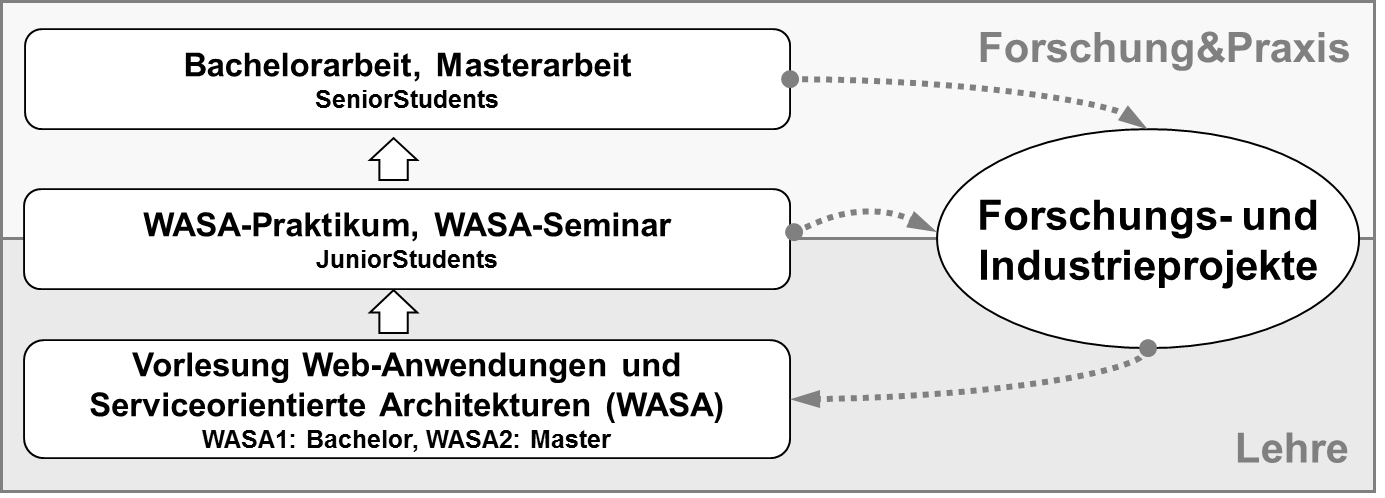
\includegraphics[width=0.8\textwidth]{images/lehre_kreislauf.png}
	\caption{Lehre-Forschung \& Praxis-Kreislauf}
	\label{fig:lehre}
\end{figure}

\begin{table}
	\centering
	\begin{tabular}{ | l | p{7cm} | }
		\hline
		ServiceGroup & Dienstleistung \\
		\hline
		 CoreServiceGroup & Campus-Informationen und Navigation \\
	 	\hline
	 	SCbInfoServiceGroup (SCbSG) & Hörsaal-Informationen für Studierende mit Beeinträchtigung \\
	 	\hline
	 	 StudAdviceTicket (StuSG) & Studierendenberatungs-Anmeldung \\
	 	\hline
	 	WorkspaceServiceGroup (WorSG) & Arbeitsplatz-Suche und -Reservierung \\
	 	\hline
	 	BaMaThesisAdminSG (BaMSG) & Abschlussarbeitenverwaltung \\
	 	\hline
	\end{tabular}
	\caption{ServiceGroups in SmartCampus}
	\label{tab:smartcampus-servicegroups}
\end{table}

\subsection{Quellcode}
\vspace{0.5cm}
\begin{lstlisting}[caption = {Vorlage für eine Story und Szenarien nach BDD}, label = {lst:bdd-stories-szenarien-template}, style = kit-cm, language = Gherkin]
Title (one line describing the story)
 
Narrative:
As a [role]
I want [feature]
So that [benefit]
 
Acceptance Criteria: (presented as Scenarios)
 
Scenario 1: Title
Given [context]
  And [some more context]...
When  [event]
Then  [outcome]
  And [another outcome]...
 
Scenario 2: ...
\end{lstlisting}


\glsresetall
\chapter{Grundlagen}
Dieses Kapitel beinhaltet Informationen, die zum grundlegenden Verständnis der Inhalte der Arbeit erforderlich sind. Die Informationen werden weitestgehend "wertfrei" dargestellt. Beispiele sind:

\begin{itemize}
	\item Grundbegriffe
	\item Einführung in grundlegenden Konzepte, Rahmenwerke, Architekturen, Methoden, Algorithmen, 
	\item Wichtige Standards, Technologien, Werkzeuge
	\item Beschreibung des betrachteten Szenarios
	\item ... 
\end{itemize}
\glsresetall
\chapter{Stand der Technik}
In dieses Kapitel fließen ganz wesentlich die Ergebnisse der Literaturanalyse ein. Es bietet sich an, die in der Einleitung eingeführte Struktur hier wieder aufzugreifen.

Im Gegensatz zu Kapitel 2 werden die Inhalte dieses Kapitels in einer argumentativen und wertenden Form dargestellt.

Kapitel 4 bis 4+n sind die zentralen konzeptionellen Kapitel der Arbeit, in denen die er-zielten Ergebnisse beschrieben werden.

Kapitel 4+n+1 kann die Beschreibung eines erstellten Prototyps (oder eines sonstigen Tragfähigkeitsnachweises) beinhalten. In diesem Zusammenhang ist abzuwägen, ob nicht anstelle eines eigenen Kapitels eine Aufteilung der Inhalte in die vorhergehenden Kapitel sinnvoll sein könnte.
% TODO create chapter files and remove this placeholders
% TODO glsresetall should be called before every chapter to explain each acronym again on first appearence
\chapter{Erstes Inhaltskapitel}
\chapter{Weitere(s) Inhaltskapitel}
%
\glsresetall
\chapter{Projektteam-Arbeiten}
Üblicherweise erfolgt die Bearbeitung eines Masterarbeitsthemas bei \gls{CM} im Rahmen eines Projektteams. Der die Masterarbeit erstellende Studierende übernimmt hierbei eine anleitende und ko-betreuende Aufgabe. Dieses üblicherweise vorletzte Kapitel der Masterarbeit dient dazu, die durchgeführten Arbeiten strukturiert zu beschreiben. Inhalte des Kapitels sind:

\begin{itemize}
	\item Inhaltliche Eingrenzung der vom Projektteam zu leistenden Arbeiten (Themengebiet, Gesamtaufgabe, Ziele)
	\item Planung der Einarbeitungsphase
	\item Zusammensetzung des Teams
	\item Vertiefende von den einzelnen Teammitgliedern bearbeitete Aufgaben
	\item Wichtige im Projektteam erarbeitete Ergebnisse
	\item ...
\end{itemize}

%
% add appendix
%

\chapter{Anhang}
\chaptermark{Anhang} 
\renewcommand{\thesection}{\Alph{section}}

%
% Abkürzungen
%

\setglossarysection{section}
\setglossarystyle{alttree}
\glssetwidest{SAMPLETE}
\printglossary[numberedsection, nonumberlist, type=\acronymtype, title=Abkürzungsverzeichnis]
\clearpage
\chaptermark{Anhang}

%
% Abbildungsverzeichnis
%

\makeatletter\newcommand{\lofwithouttitle}{\@starttoc{lof}}\makeatother
\section{Abbildungsverzeichnis}
\lofwithouttitle
\clearpage

%
% Tabellenverzeichnis
%

\makeatletter\newcommand{\lotwithouttitle}{\@starttoc{lot}}\makeatother
\section{Tabellenverzeichnis}
\lotwithouttitle 
\clearpage

%
% Quelltextverzeichnis
%

\makeatletter\newcommand{\lolwithouttitle}{\@starttoc{lol}}\makeatother
\section{Quelltextverzeichnis}
\lolwithouttitle
\clearpage

%
% Literaturanalyse
%

\section{Literaturanalysen}

Angabe der Literaturanalyse zu den wichtigsten Dokumenten, die in der Diplomarbeit referenziert wurden. Die analysierten Dokumente sind gemäß ihrer Relevanz zu ordnen. Die Literaturanalysen zu den drei ersten Dokumenten gehen verstärkt in die Bewertung der Diplomarbeit ein.

%\renewcommand*\descriptionlabel[1]{\hspace\labelsep\normalfont #1}

% TODO copy default analysis
\subsection{Titel der analysierten Publikation}
\begin{description}[leftmargin=!,labelwidth=\widthof{\bfseries \cite{Be02}}]
	\item [\cite{Be02}] {Vorname Name: Titel der analysierten Publikation, weitere Angaben.}
\end{description}

\textbf{Inhalte}
Was sind die zentralen Inhalte (Themen, interessante Aussagen, Botschaften, Fragestellungen), die in der Arbeit (d.h., in der analysierten Literatur) behandelt werden?
\begin{description}[leftmargin=!,labelwidth=\widthof{\bfseries [(I1)]}]
	\item [(I1)] {...}
	\item [(I2)] {...}
	\item [(I3)] {...}
\end{description}

\textbf{Defizite} 
Welche Defizite bestehender Arbeiten und Lösungen werden als Motivation der eigenen Lösungen genannt?
\begin{description}[leftmargin=!,labelwidth=\widthof{\bfseries [(I1)]}]
	\item [(D1)] {...}
	\item [(D2)] {...}
	\item [(D3)] {...}
\end{description}

\textbf{Prämissen}
Welche Einschränkungen und Vorgaben werden hinsichtlich der eigenen Lösungen ge-macht?
\begin{description}[leftmargin=!,labelwidth=\widthof{\bfseries [(I1)]}]
	\item [(P1)] {...}
	\item [(P2)] {...}
	\item [(P3)] {...}
\end{description}

\textbf{Lösungen}
Was sind die eigenen Lösungen?
\begin{description}[leftmargin=!,labelwidth=\widthof{\bfseries [(I1)]}]
	\item [(L1)] {...}
	\item [(L2)] {...}
	\item [(L3)] {...}
\end{description}

\textbf{Nachweise}
Welche Nachweise (Evidence) werden hinsichtlich der Tragfähigkeit der eigenen Lösun-gen geliefert?
\begin{description}[leftmargin=!,labelwidth=\widthof{\bfseries [(I1)]}]
	\item [(N1)] {...}
	\item [(N2)] {...}
	\item [(N3)] {...}
\end{description}

\textbf{Offene Fragen} 
Welche Fragen sind noch ungelöst geblieben bzw. stellen sich dem Leser?
\begin{description}[leftmargin=!,labelwidth=\widthof{\bfseries [(I1)]}]
	\item [(O1)] {...}
	\item [(O2)] {...}
	\item [(O3)] {...}
\end{description}

\textbf{Sonstiges} \\
Punkte, die in keine der oben genannten Kategorien passen



\clearpage

%
% Glossar
%

\glossarystyle{altlist}
\printglossary[title=Glossar, type=main, nonumberlist]
\clearpage
\chaptermark{Anhang}

%
% Literaturverzeichnis
%

\makeatletter
\renewenvironment{thebibliography}[1]
     {\section{\bibname}
      \list{\@biblabel{\@arabic\c@enumiv}}
           {\settowidth\labelwidth{\@biblabel{#1}}
            \leftmargin\labelwidth
            \advance\leftmargin\labelsep
            \@openbib@code
            \usecounter{enumiv}%
            \let\p@enumiv\@empty
            \renewcommand\theenumiv{\@arabic\c@enumiv}}
      \sloppy
      \clubpenalty4000
      \@clubpenalty \clubpenalty
      \widowpenalty4000
      \sfcode`\.\@m}
     {\def\@noitemerr
       {\@latex@warning{Empty `thebibliography' environment}}%
      \endlist}
\makeatother

\bibliography{literatur}

\bibliographystyle{cmnat}

%
% Einbinden eines PDF-Anhang
%
%\includepdf[pages=1, pagecommand={\section{Abschnitt} \thispagestyle{scrheadings}}, scale=0.7]{chapters/anhang.pdf}
%\includepdf[pages=2-last, pagecommand={\thispagestyle{scrheadings}}, scale=0.7]{chapters/anhang.pdf}

%==============================================================================

\end{document}